\chapter{ПЕРЕЧЕНЬ СТЕНДОВОГО ОБОРУДОВАНИЯ}\label{app:equipment_list}
В данном приложении представлен перечень основного оборудования, использованного при
создании экспериментального стенда для исследования позиционного пневмопривода с дискретным управлением.

\begingroup
\centering
\small
\captionsetup[table]{skip=7pt} % смещение положения подписи
\begin{longtable}[c]{|m{0.2\textwidth}|m{0.3\textwidth}|m{0.25\textwidth}|}
	\caption{Перечень оборудования экспериментального стенда}\label{tab:equipment_list}
	\\[-0.45\onelineskip]
	\hline
	\textbf{Наименование}                                    & \textbf{Основные характеристики} & \textbf{Внешний вид} \\
	\hline
	\endfirsthead

	\caption*{Продолжение таблицы~\thetable}                                                                           \\[-0.45\onelineskip]
	\hline
	\textbf{Наименование}                                    & \textbf{Основные характеристики} & \textbf{Внешний вид} \\
	\hline
	\endhead
	\hline
	\endfoot
	\hline
	\endlastfoot
	Пневмоцилиндр DSNU-32-350-PPV-A                          &
	Диаметр поршня: 32 мм;
	Ход: 350 мм;
	Диаметр штока: 12 мм;
	Макс. рабочее давление: \num{1.0} МПа;
	Макс. скорость: \num{1.5} м/с.
	                                                         &
	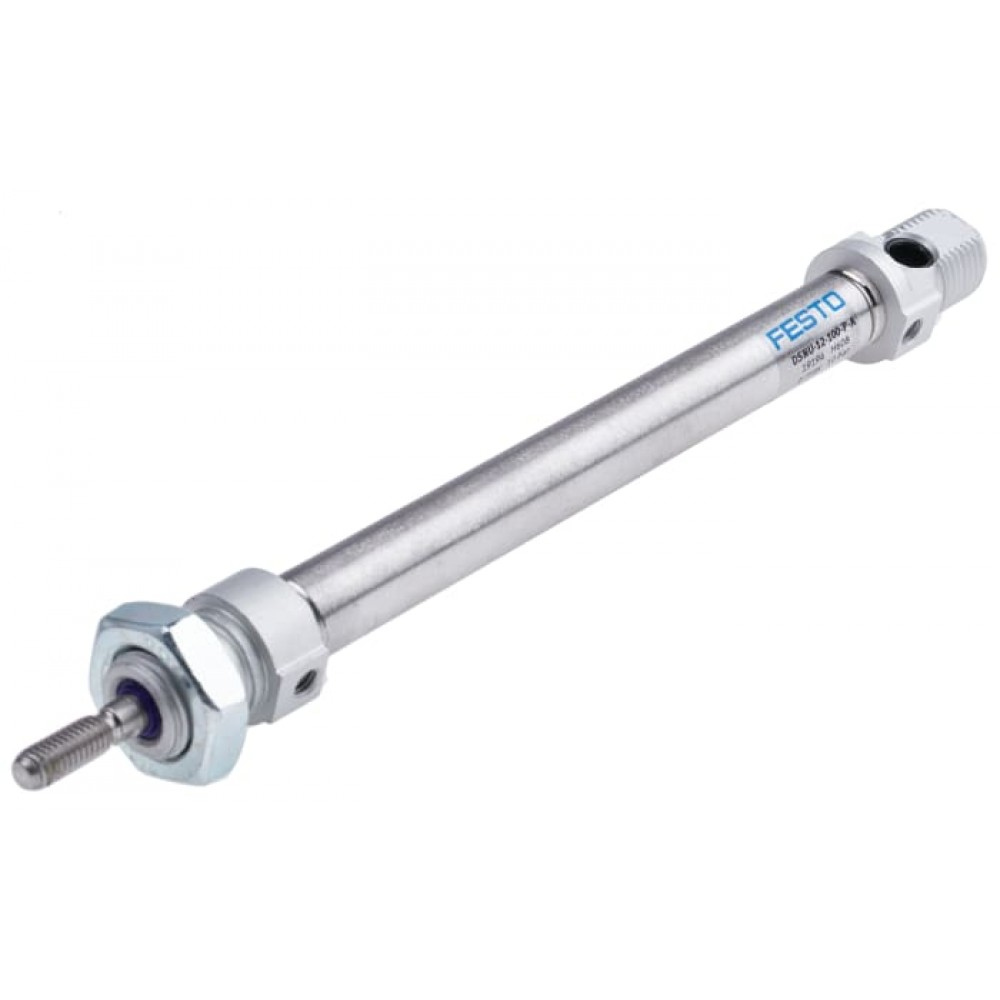
\includegraphics[width=4cm]{appendix/cylinder.jpg}                                                                 \\
	\hline
	Распределитель Camozzi AA31-0C2                          &
	Тип: 3/2 NC;
	Пропускная способность: 750 Нл/мин;
	Время переключения: 20 мс;
	Рабочее напряжение: 24В DC;
	Потребляемая мощность: \num{1.8} Вт.
	                                                         &
	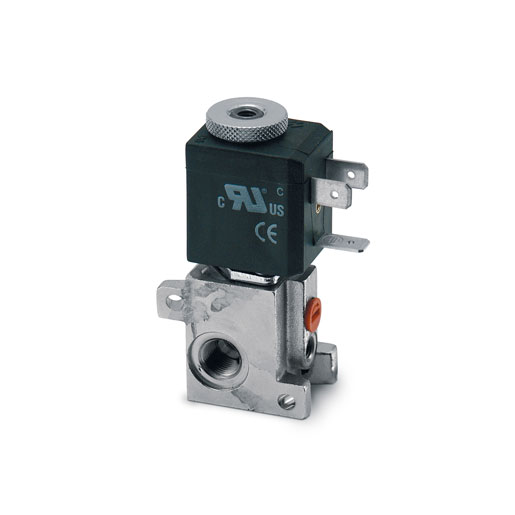
\includegraphics[width=4cm]{appendix/AA31-0C2+.jpg}                                                                \\
	\hline
	Датчик давления Festo SPAU-P10R-H-G18FD-L-PNLK-PNVBA-M8U &
	Диапазон измерения: 0–10 бар;
	Выход: аналоговый сигнал;
	Точность: $\pm \num{0.5}$\% FS;
	Рабочее напряжение: 24В DC.
	                                                         &
	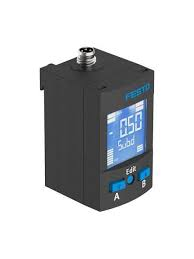
\includegraphics[width=4cm]{appendix/spau_pressure_sensor.jpg}                                                     \\
	\hline
	Датчик положения Festo MLO-POT-450-TLF                   &
	Тип: потенциометр;
	Диапазон измерения: 0~--~450 мм;
	Рабочее напряжение: 10В DC.
	                                                         &
	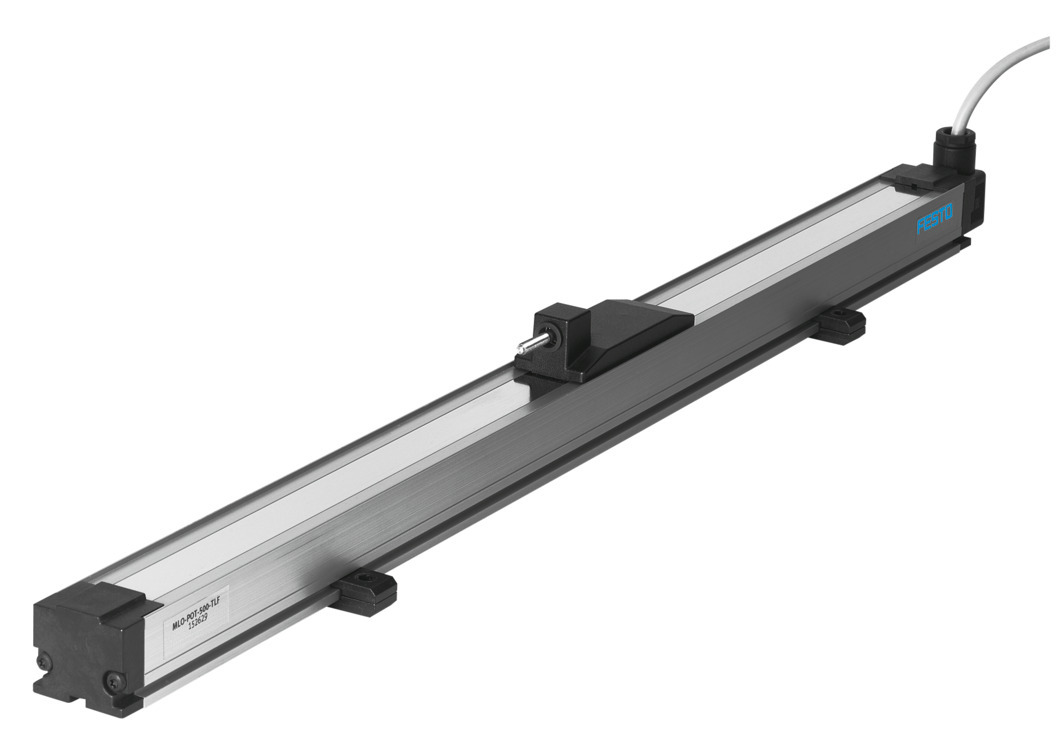
\includegraphics[width=4cm]{appendix/festo_position_sensor.jpg}                                                    \\
	\hline
	STM32F767ZI                                              &
	Микроконтроллер ARM Cortex-M7;
	Тактовая частота: 216 МГц;
	Флеш-память: 2 МБ;
	SRAM: 512 КБ;
	Набор периферии: USB, Ethernet, CAN, ADC.
	                                                         &
	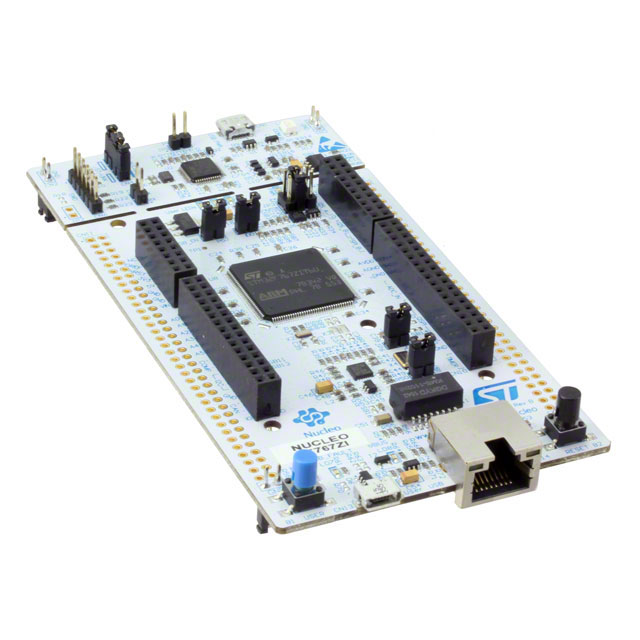
\includegraphics[width=4cm]{appendix/stm32f767zi.jpg}                                                              \\
	\hline
	Raspberry Pi 5                                           &
	Процессор: Broadcom (до \num{1.8} ГГц);
	Оперативная память: 4/8 ГБ;
	Интерфейсы: USB \num{3.0}, Gigabit Ethernet, WiFi, Bluetooth;
	Поддержка 4K видео.
	                                                         &
	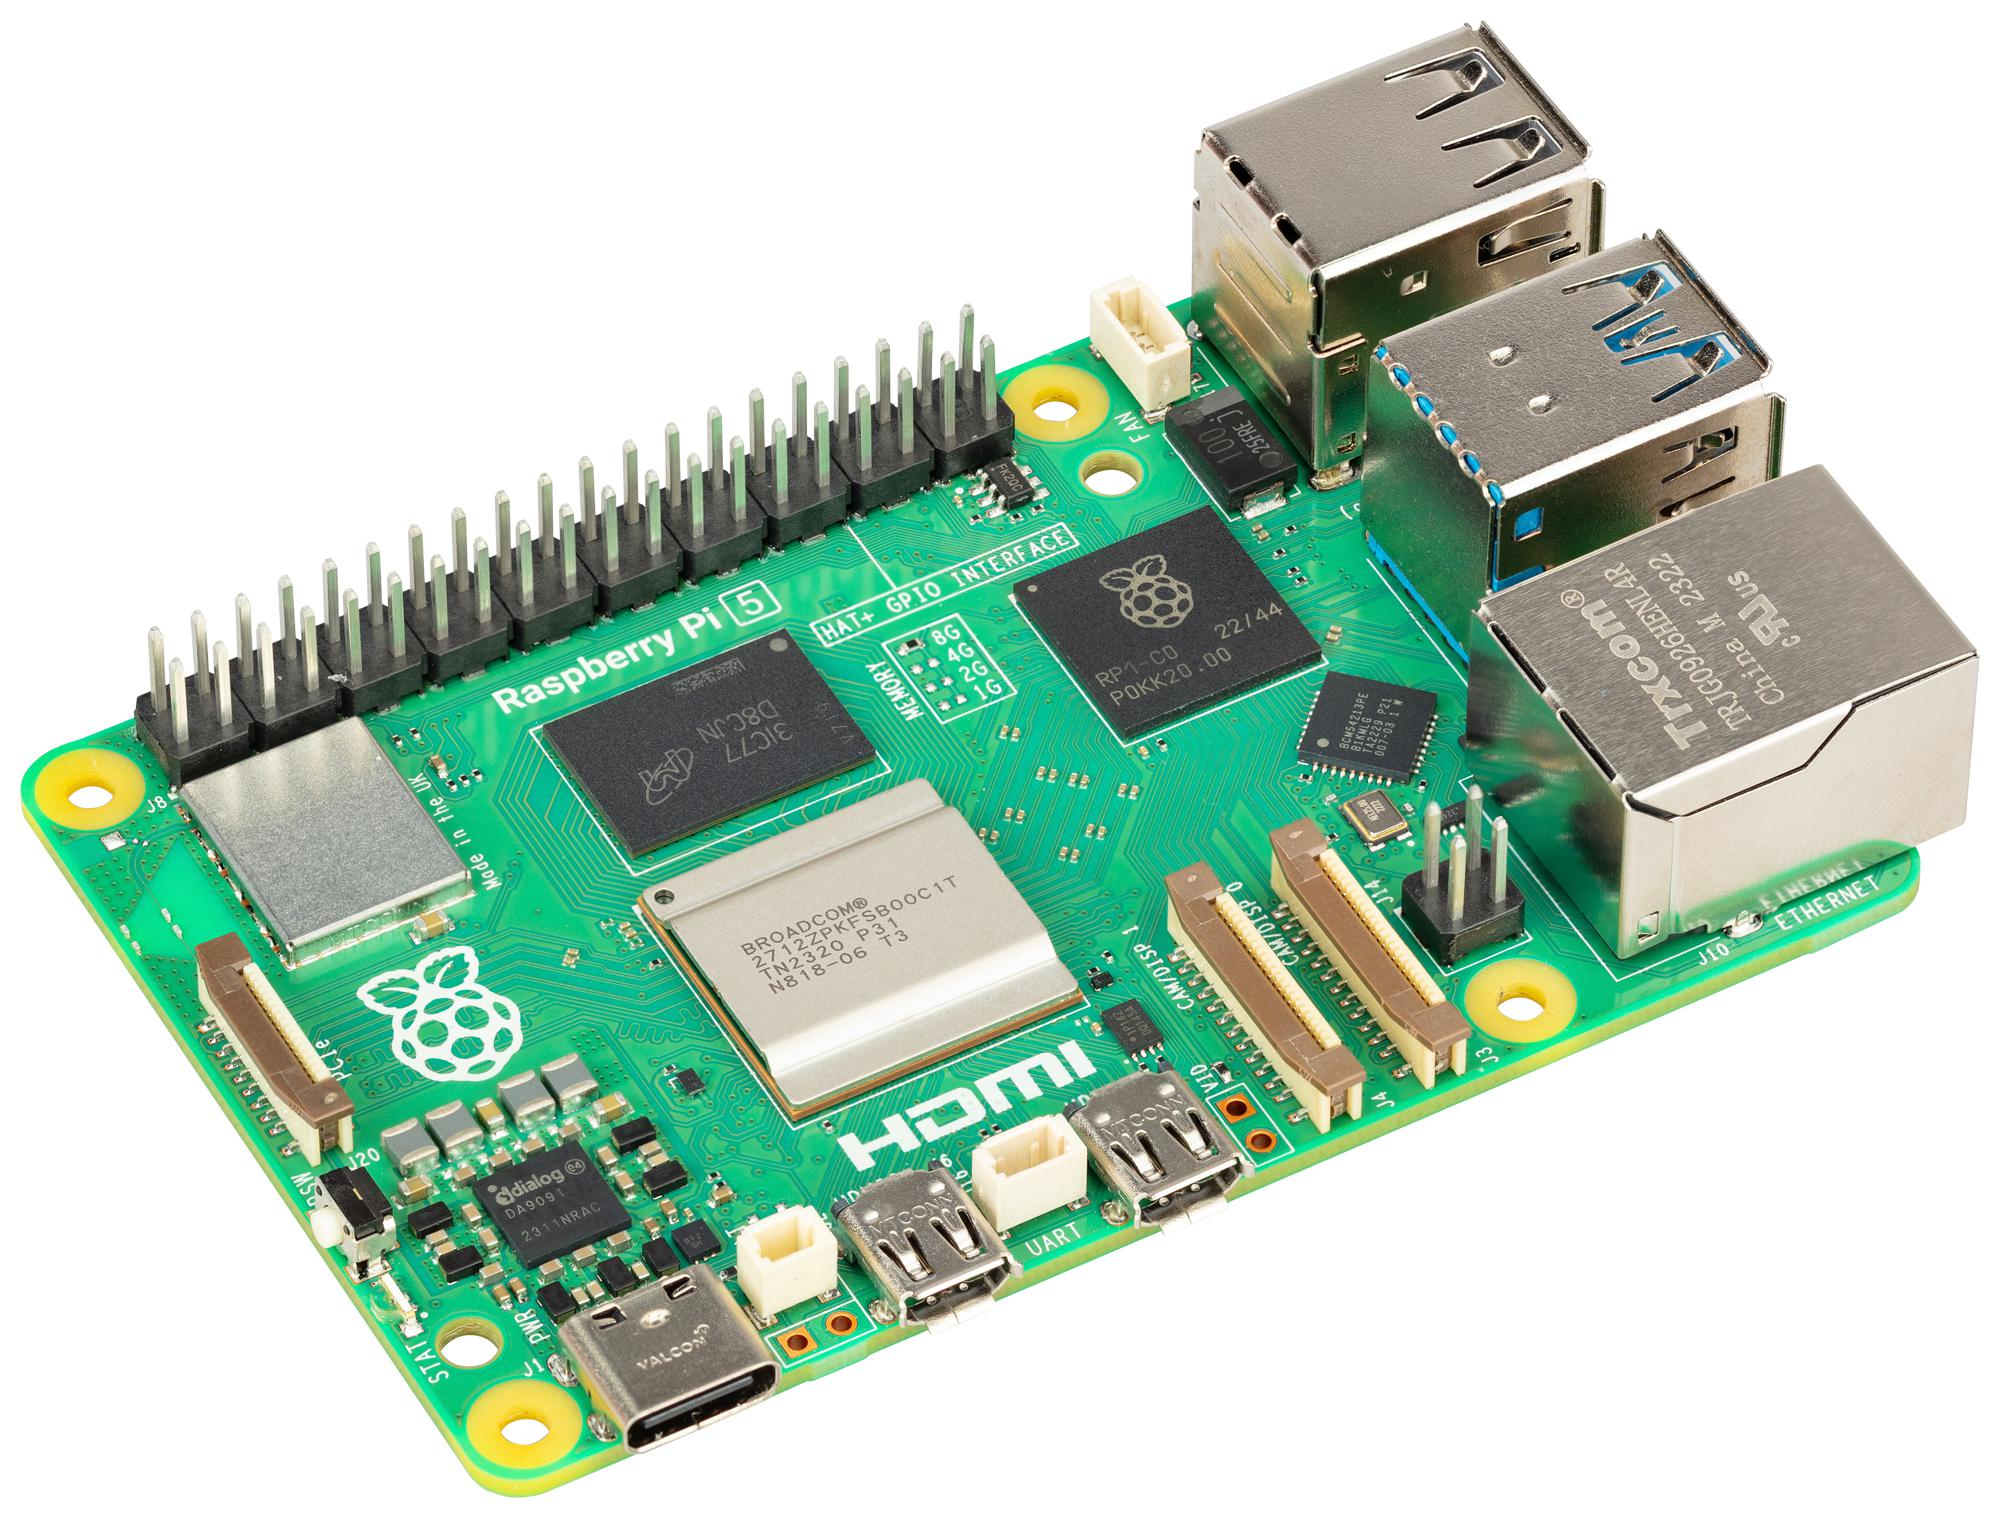
\includegraphics[width=4cm]{appendix/raspberrypi5.jpg}                                                             \\
	\hline
	АЦП ADS1256                                              &
	Разрешение: 24 бит;
	Скорость выборки: до 30 кГц;
	Интерфейс: SPI;
	Много канальный.
	                                                         &
	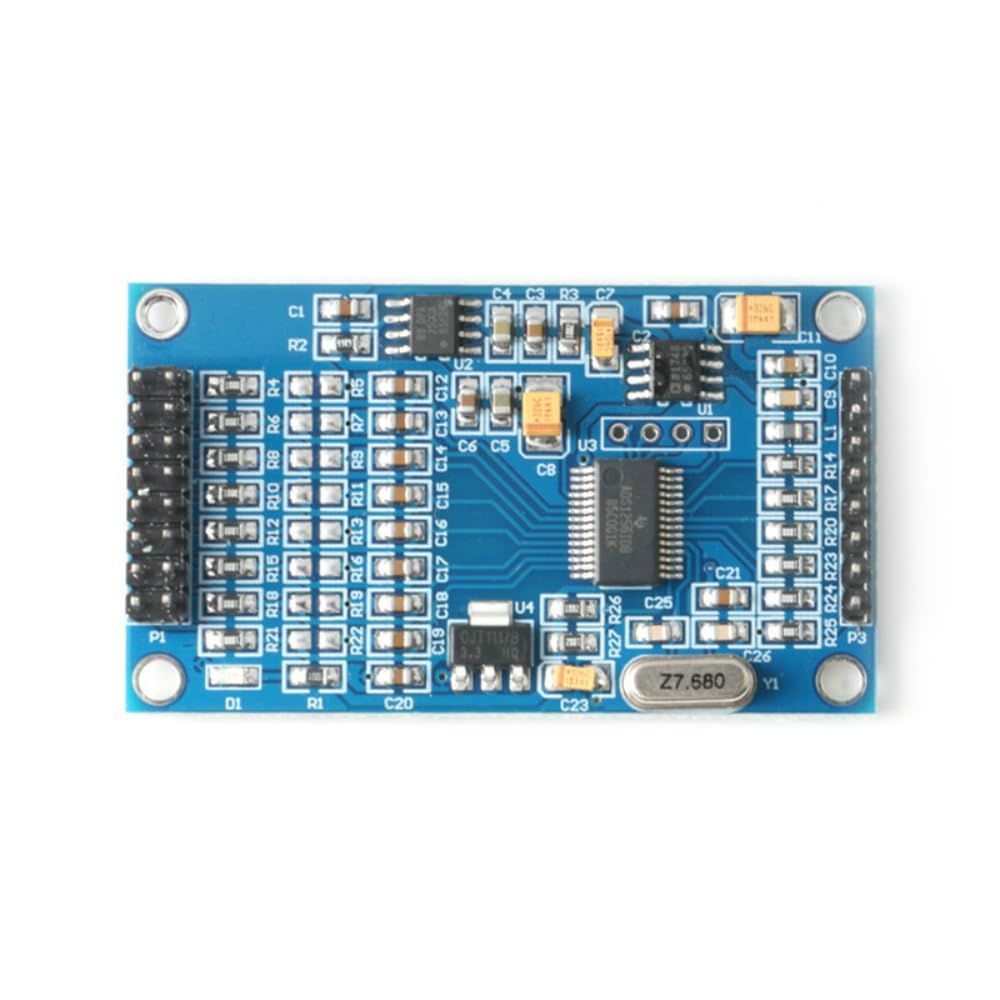
\includegraphics[width=4cm]{appendix/ads1256.jpg}                                                                  \\
	\hline
\end{longtable}
\normalsize% возвращаем шрифт к нормальному
\endgroup